\section{Experiments}

\subsection{Experimental setup}

Our experiments all use the Llama \citep{Llama} architecture trained on WikiText-103~\citep{WikiText103} (excepting the large-scale runs in \Cref{sec:fp8_training}). We apply current best-practice LLM training techniques from the literature (full settings are given in \Cref{tab:experiment_defaults}). In accordance with our analysis of settings for \mut\ in \Cref{sec:challenges:mut}, we remove parameters from norm layers, use independent AdamW, and avoid training on too many epochs for both \umup\ and \mup\ for the sake of fair comparison.

\subsection{Quantifying hyperparameter interdependence} \label{sec:experiments:hp_independence}

Our principled approach to HPs (\Cref{sec:umup:principled_hps}) contains the requirement that their optimal values should depend minimally on the value of other HPs. We now investigate this empirically, conducting a 2D sweep over every pair of HPs for \mup\ and \umup, shown in \Cref{fig:additional_experiments:mult_grid_mup,,fig:additional_experiments:mult_grid_umup} respectively.

To derive an empirical measure of HP dependency, we introduce the notion of \textit{transfer error} (see \Cref{alg:transfer_error}). This considers a pair of HPs, with one `fixed' and the other for `transfer'. We take the best value of the transfer HP for each non-optimal value of the fixed HP, and use it with the optimal value of the fixed HP. The transfer error is the difference between the losses obtained and the minimum loss. \Cref{fig:experiments:transfer_error} shows this measure for each pair of HPs under \mup\ and \umup, reflecting the improvement in HP dependency as a result of our scheme. This gives \umup\ a reduced risk of small transfer errors leading to large degradations, and the potential to sweep HPs in a more separable way.

\begin{figure}[t]
    \vspace{-1em}
    \centering
    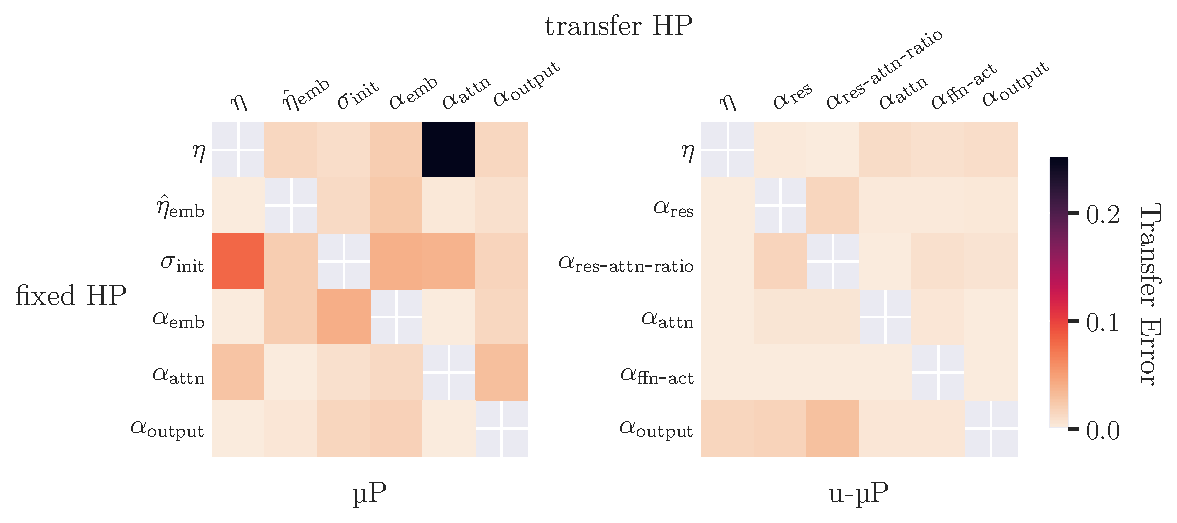
\includegraphics[width=\textwidth]{arXiv/figures/hp_pair_dependencies_val.pdf}
    \caption{A visualization of the dependencies between pairs of HPs under each scheme. Transfer error measures the extent to which the optimal value of the transfer HP depends on the fixed HP (see \Cref{alg:transfer_error}). On average, \mup\ has a transfer error of 0.03, whereas \umup\ has 0.005.}
    \label{fig:experiments:transfer_error}
\end{figure}

\subsection{Hyperparameter search} We now leverage this improved separability of HPs for the purpose of efficient sweeping. In \Cref{fig:fig1}~(a) we conduct a standard random search for \mup\ and \umup, along with the independent search outlined in \Cref{sec:umup_hp_search} (and \Cref{app:umup_hp_search_algorithm}). We observe the following:

\begin{enumerate}
    \item For \umup\ the LR-sweep phase of independent search alone is sufficient to reach near-optimal loss (totaling 9 runs). During this phase other HPs are fixed at 1, which for \umup\ means that the inputs to operations are generally unit-scaled.

    \item Consequently, we conclude that unit scale at initialization is close to the ideal scaling for effective learning here. This is not a property we asserted a priori, nor do we argue that it necessarily holds for other training setups and models; hence why we still provide a set of extended HPs to be swept.

    \item In contrast \mup\ still requires non-LR HPs to be swept to attain a reasonable loss. Unlike \umup, fixing HPs at 1 results in arbitrarily-scaled inputs, which appear to result in worse training.

    \item The `combined mults' phase causes the loss to spike for \mup. This is due to the HP dependencies shown in \Cref{fig:experiments:transfer_error}, which mean HPs cannot be swept independently and used together. Conversely, lower dependence means this can be done for \umup, making random search unnecessary.
\end{enumerate}

\subsection{Hyperparameter transfer}

% As \umup\ follows the \mup\ parametrization rules (with the exception of the embedding LR scaling rule in \Cref{sec:umup:emb_lr_rule}), we still expect it to satisfy the transfer properties of \mup. In fact, \umup's transfer properties are generally better than those of the \mup\ baseline, thanks to our unit-scale criterion and careful HP design.

We demonstrate the transfer of LR across width in \Cref{fig:fig1} (b), of the other extended HPs across width in \Cref{fig:lr_transfer}, and of LR across training steps, batch size and depth in \Cref{fig:experiments:hp_transfer_over_width}. We find that:

\begin{enumerate}
    \item The optimal LR is constant for all widths under \umup, from 128 to 4096.

    \item The optimal LR is also approximately constant for training steps, batch size and depth. This means we can scale our proxy model down across all these axes and maintain LR transfer. Of these, width appears the most stable and depth the least.

    \item Whereas \mup\ sees diminishing returns for larger widths, \umup\ continues to benefit from width, with the 2048 \umup\ model matching the 4096 \mup\ model. We attribute this primarily to our improved embedding LR rule.

    \item Non-LR HPs also have approximately constant optima across width under \umup. This is not true for \mup, where $\hat{\eta}_\mathrm{emb}$ has poor transfer due to the embedding scaling rule issue identified in \Cref{sec:umup:emb_lr_rule}, along with $\sigma_\mathrm{init}$ which in \Cref{sec:challenges:which_hps} we argue should not be grouped across all weights (and drop from the \umup\ HP scheme).

    \item The optimal values found for non-LR HPs are all close to 1. In practice this means that dropping these HPs entirely is potentially viable for similar models and training setups.
\end{enumerate}

\begin{figure}[t]
    \centering
    \begin{subfigure}{\textwidth}
        \centering
        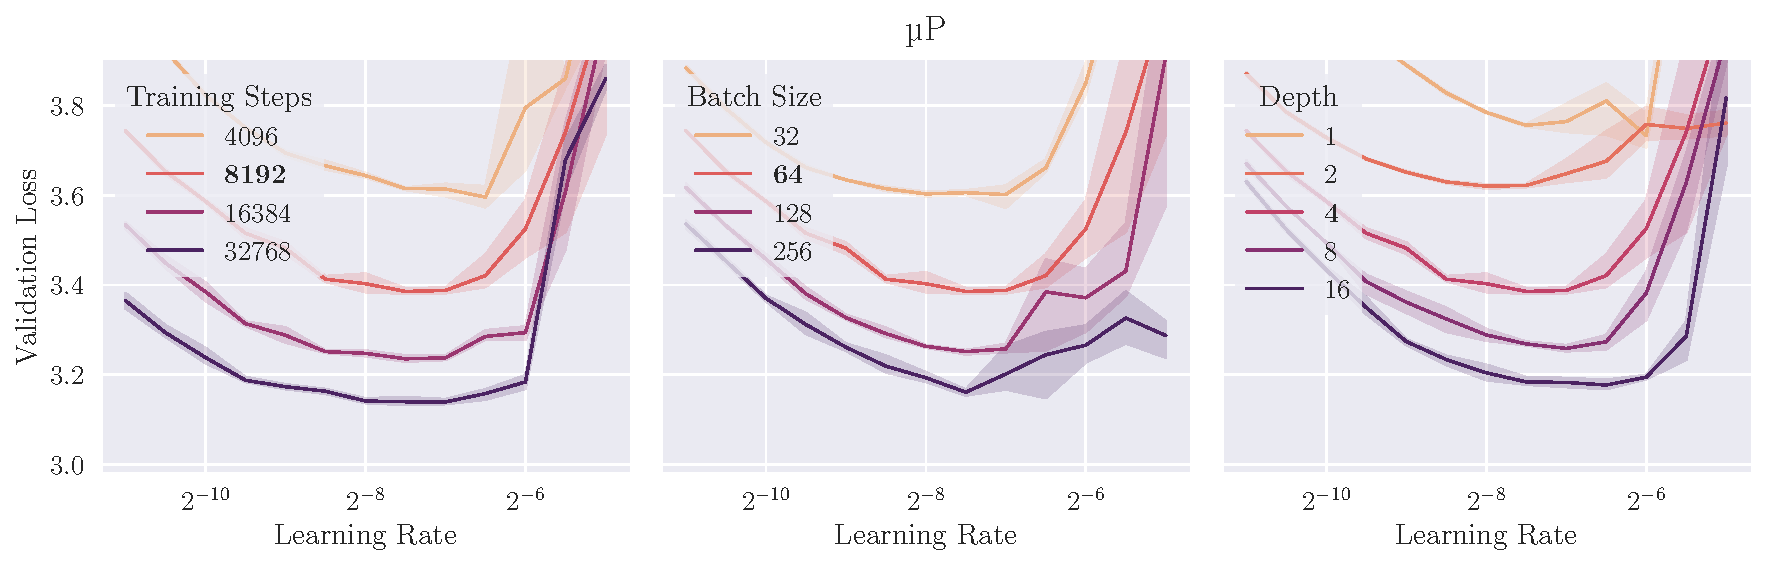
\includegraphics[width=\textwidth]{arXiv/figures/lr_transfer_mup.pdf}
    \end{subfigure}
    \begin{subfigure}{\textwidth}
        \centering
        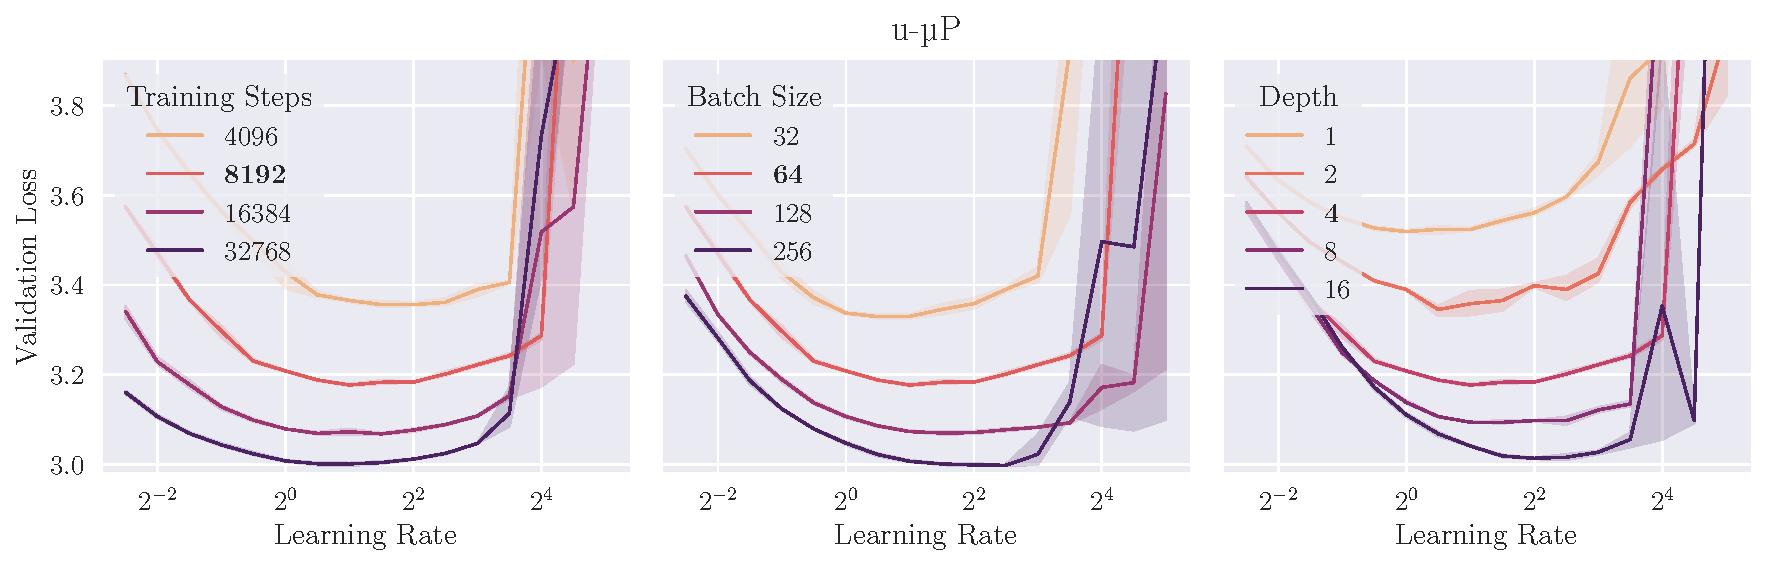
\includegraphics[width=\textwidth]{arXiv/figures/lr_transfer_u-mup.pdf}
    \end{subfigure}
    \caption{Learning rate transfer for \mup{} (top) and \umup{} (bottom), over training steps, batch size and depth. See \Cref{fig:fig1}~(b) for transfer over width. The \textbf{default} shape parameter for other panels is shown in bold. The shaded area shows the $95\%$ confidence interval for the mean.}
    \label{fig:lr_transfer}
\end{figure}

\subsection{FP8 training} \label{sec:fp8_training}

In this section we justify the simple mixed-precision scheme described in \Cref{sec:umup:low_prec_training} and demonstrate that it can be used to train \umup\ models out-of-the-box.

\paragraph{Proof-of-concept} \Cref{fig:numerics:scale} shows the RMS of all linear layer inputs for a moderately sized transformer. RMS captures the larger of the mean and scale of a distribution, and as such is a good test of whether a tensor is likely to suffer over/underflow in low-precision. We observe that \umup\ tensors largely have RMS starting close to $1$ and remaining so at the end of training, supporting our scheme.

\Cref{fig:numerics:rms_during_training} demonstrates the scale-growth of critical tensors which our scheme is designed to accommodate, showing RMS on a per-tensor basis over steps. \Cref{fig:numerics:scale_scaling} provides further insight into this issue, showing the effect of LR, width, depth, steps and batch size on the RMS of critical tensors.

As an initial proof-of-concept we train a \umup\ model using our FP8 scheme over 8k steps, using HPs from a proxy model, as shown in \Cref{fig:fig1}~(c). We see only a small degradation versus FP32, and at this scale critical tensors can still be cast to FP8 using \texttt{E5M2}, while gradients can even use \texttt{E4M3}.

%\subsection{Numerical properties} \label{subsec:numerical_properties}

%,  Detailed analysis of these statistics is given in \Cref{app:fp8_training}, with our results supporting the central thesis of Unit Scaling: that tensors are well-scaled at initialization and largely remain so across training.

%Based on these conclusions we propose our primary FP8 scheme: for every matrix multiplication, we cast the input, weight and grad-output tensors to \texttt{E4M3}, with the exception of the inputs to FFN and self-attention final projections, which are cast to \texttt{E5M2} to accommodate their growing scale. This simply requires FP8 casts to be inserted into the model, avoiding the more complex scaling techniques used for FP8 in the literature (see \Cref{app:low_precision_and_its_trade_offs}). This is possible due to the numerical stability we see in our analysis of \umup. Additional details of our primary FP8 scheme are given in \Cref{app:fp8_scheme}.

%As we demonstrate in \Cref{subsec:large_scale}, the primary scheme needs to be slightly adapted when model size, sequence length and number of training steps increase substantially. 

%\subsection{FP8 training at smaller scale} \label{sec:experiments:fp8}

%We now show that \umup\ can indeed be trained in our primary FP8 scheme in a smaller-scale setting (in terms of training tokens, rather than model-size). We note that our aim here is a proof-of-concept that this form of low-precision training can be done without degradation, not a demonstration of improved throughput which we leave to future work. To investigate the question of the potential benefits of FP8 training, \Cref{app:scaled_mm_benchmarking} shows results for micro-benchmarking low-precision matmuls. We find that the addition of scaling factors adds no overhead, making our \umup\ modifications essentially `free'.

%\Cref{fig:fig1} (c) demonstrates the application of our FP8 scheme to model-training at width 4096. We use exactly the HPs suggested by the sweep in \Cref{fig:fig1} (a), but transferred to the larger model-width. \mup\ fails entirely under our FP8 scheme due to gradient underflow, reflecting the requirement for different, and likely more complex scaling scheme. In contrast, \umup\ trains in FP8 with only a small increase in validation loss versus the full-precision baseline.

\begin{figure}[t]
    \centering
    \begin{subfigure}{.46\textwidth}
        \centering
        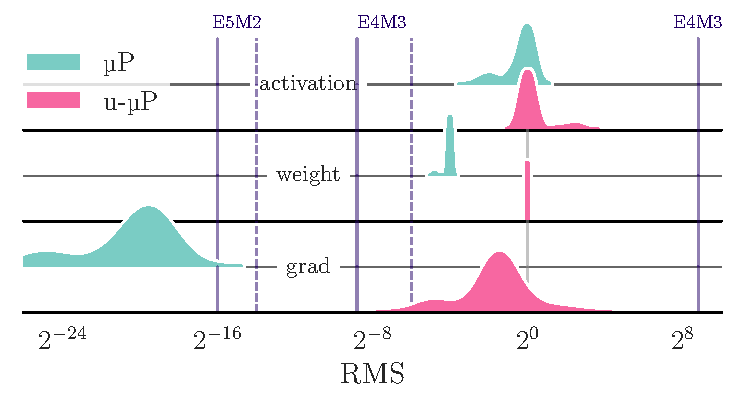
\includegraphics[width=\textwidth]{arXiv/figures/rms_at_init.pdf}
    \end{subfigure}
    \begin{subfigure}{.46\textwidth}
        \centering
        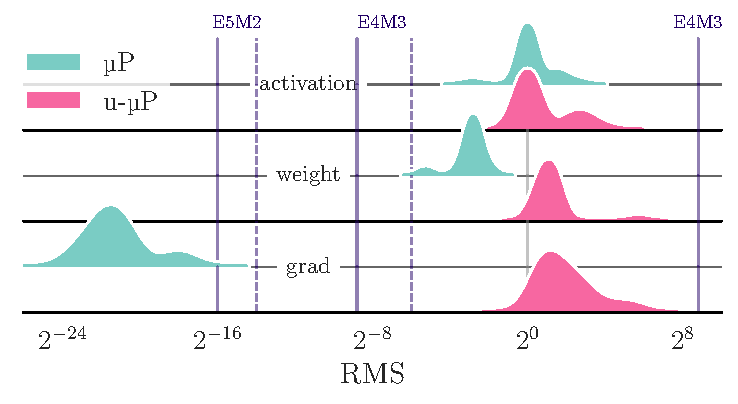
\includegraphics[width=\textwidth]{arXiv/figures/rms_end_training.pdf}
    \end{subfigure}
    \caption{Per-tensor $\mathrm{RMS} = \sqrt{\sigma^2 + \mu^2}$ across \umup\ and \mup\ models at initialization (left) and after training (right). \umup\ tensors have RMS that starts close to $1$ and remains within E4M3 range at the end of training. Dashed and solid red lines show each format's min. normal and subnormal values.}
    \label{fig:numerics:scale}
\end{figure}

%\subsection{FP8 training at large-scale} \label{subsec:large_scale}

\paragraph{Larger scale} Next we consider a more realistic training scenario \footnote{The training codebase used for our larger-scale experiments can be found at the following url \url{https://github.com/Aleph-Alpha/scaling}. We have also released model checkpoints, which are available at \url{https://huggingface.co/Aleph-Alpha}.}.
% \footnote{The large scale experiments were run on a separate code base optimized for distributed training that will be made available in the near future.}
Using the same architecture, and following the steps set out in our \umup\ user-guide (\Cref{app:using_umup_guide}), we train our target models on 300B tokens of the SlimPajama dataset \citep{SlimPajama} (see \Cref{app:large_model_training} for training details).

We begin with an independent search (\Cref{sec:umup_hp_search}) over our \umup\ proxy model's HPs. Here we make the following observations:
\begin{enumerate}
    \item When using a relatively small proxy model (8 layers and 512 width), the HP-loss landscape is rather noisy. By doubling the width we can discern optimal HP values more clearly.
    \item The most important HPs are $\eta$ and $\alpha_\mathrm{res\text{-}attn\text{-}ratio}$. All others can be left at the default of $1$.
    \item The optimal values of these HPs are $\eta = 2^{3.5}$ and $\alpha_\mathrm{res\text{-}attn\text{-}ratio} = 2^{-2.0}$ and thus differ non-trivially from the observed HPs in our smaller-scale experiments.
\end{enumerate}

We then train \umup\ models of approximately 1B, 3B and 7B parameters, using our FP8 mixed-precision scheme (see \Cref{sec:umup:low_prec_training}). We also train two baselines at each size: the first is a BF16 version of our \umup\ models, and the second is a set of SP models using the weight init scheme from the Pythia model family~\citep{Pythia} and the LR scheme from Llama 3~\citep{LLAMA3}, scaling inversely with width and using a LR of 3e-4 at 7B scale.
The loss curves are shown in \Cref{fig:scaleup}. All FP8 runs converge and show no significant loss degradation. In comparison to SP, the \umup\ models have a qualitatively different training curve with a higher loss for most of training that catches up in latter stages, hinting at a fundamentally different optimization trajectory. In terms of downstream performance, both of the \umup\ 7B models are competitive with SP. In particular, the scores of the FP8 model are mostly on par with the BF16 models (see \Cref{tab:eval_results}).

%We also record the magnitude of tensors in the model during training (\ce{TODO: include figure }). Some of the critical layers show a significant scale growth over time, which makes it impossible to naively cast them to FP8. On the other hand, the non-critical tensor scales are very stable across training time, and model size. This is strong evidence for \umup\ FP8 to work at even larger scales.

% . We also observe that using purely the \texttt{E4M3} format in the `non-problematic' layers leads to divergence as well, whereas the hybrid scheme of using \texttt{E4M3} for the activation and the weight and \texttt{E5M2} for the output gradient is stable.
%To tackle the layers that exhibit scale growth, we fit them with a lightweight form of dynamic rescaling, leaving the rest of the model untouched. 

%The dynamic rescaling works as follows: Before the matrix multiplication, we normalize the input by its standard deviation and divide the result by the same scale afterwards, while ignoring both of these operations in the backward computation. We emphasize that this is still considerably less complex than the per-tensor scaling strategy that is usually required for FP8 training.

%Using this refined FP8 scheme we perform two series of experiments:
%\begin{enumerate}
  %  \item On the 1B scale, we train a comparable SP model adopting the learning rate and initialization scheme from the Pythia model family~\citep{Pythia}, which we consider a strong established baseline. Apart from a standard training in BF16 mixed precision, we also try a simple FP8 cast and the Nvidia Transformer Engine framework~\citep{Transformer_Engine} for this baseline. We then compare these SP models to three variants of our \umup\ 1B model: One model in mixed precision, one model casting all layers except the critical ones to FP8 (our `partial' scheme in \Cref{fig:scaleup}), and one where we apply our full FP8 scheme. Overall the \umup\ models perform favorably  (see \Cref{fig:scaleup} (left)).
   % \item We train FP8 models up to 7B parameters using our full FP8 scheme. All runs converge (see \Cref{fig:scaleup} right), and we expect our method to work at larger scales still.
%\end{enumerate}


%We then train our target models using this FP8 scheme in \Cref{fig:dynamic_rescaling_losses}. At each model-size we demonstrate successful FP8 training, and expect it to work at larger scales still.

%\begin{figure}[t]
  %  \centering
  %  \begin{subfigure}{\textwidth}
  %      \centering
  %      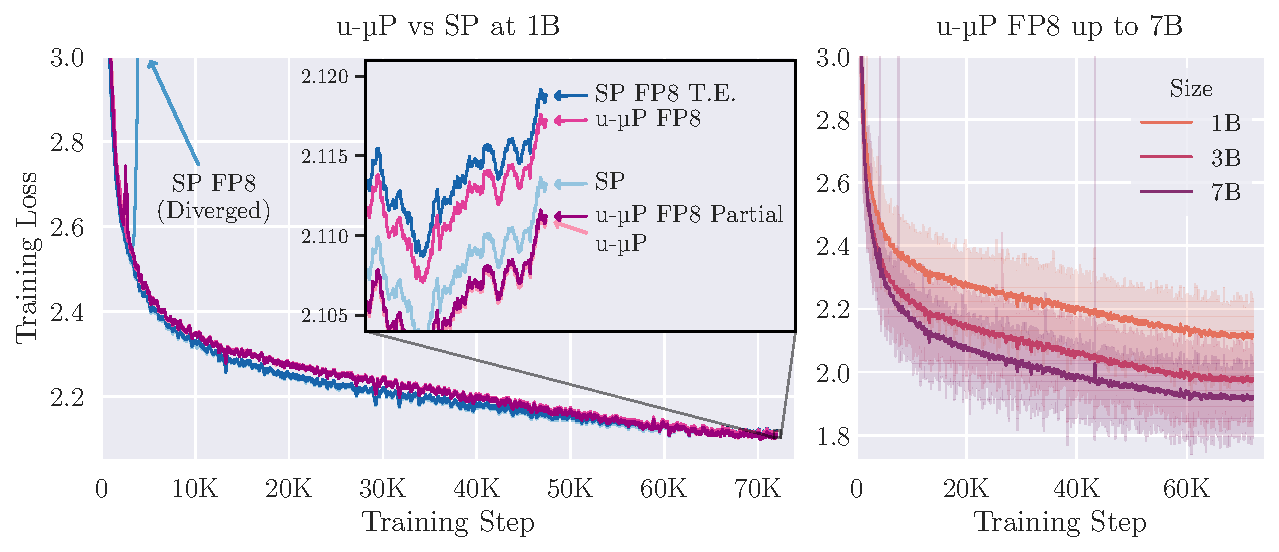
\includegraphics[width=\textwidth]{arXiv/figures/fig_scaleup.pdf}
  %  \end{subfigure}
  %  \caption{(Left) Comparison of 1B training curves for \umup\ and SP, using BF16 mixed precision vs FP8. Directly casting to FP8 causes SP to diverge, whereas \umup\ still converges and outperforms the Transformer Engine FP8 baseline (SP FP8 T.E.). Using our proposed partial FP8 scheme, \umup\ maintains nearly full performance compared to BF16 mixed precision. (Right) Loss curves from large scale training runs up to 7B using the \umup\ FP8 scheme. Both figures use a smoothed running average loss with window size 100.}
  %  \label{fig:scaleup}
%\end{figure}

\begin{figure}[t]
    \vspace{-1.5em}
    \centering
    \begin{subfigure}{0.4\textwidth}
        \centering
        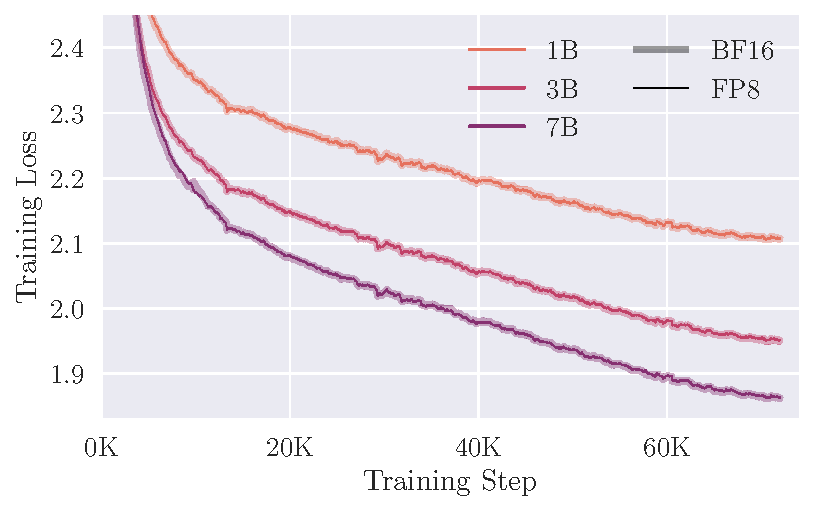
\includegraphics[width=\textwidth]{arXiv/figures/large_scale_BF16_vs_FP8.pdf}
    \end{subfigure}
    \hspace{2em}
    \begin{subfigure}{0.4\textwidth}
        \centering
        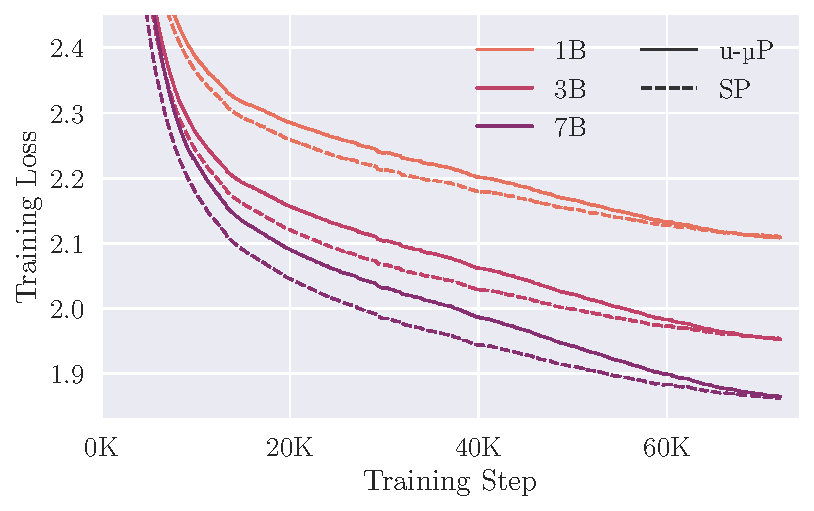
\includegraphics[width=\textwidth]{arXiv/figures/large_scale_umup_vs_sp.pdf}
    \end{subfigure}
    \vspace{-0.5em}
    \caption{Large-scale training runs. (Left) \umup\ BF16 vs \umup\ FP8. (Right) \umup\ BF16 vs SP BF16.}
    \label{fig:scaleup}
\end{figure}

\begin{table}[t] 
  \centering
  \caption{0-shot benchmark results at 7B scale.}
\begin{tabular}{llcccccc}
\toprule
Scheme & Format & MMLU & HellaSwag & OpenBook QA & PIQA & TriviaQA & WinoGr \\
\midrule
SP & BF16 & 29.6 & 52.4 & 27.8 & 76.5 & 22.2 & 63.3 \\
\umup\ & BF16 & 29.0 & \textbf{53.4} & \textbf{31.6} & 77.1 & \textbf{23.4} & 63.7 \\
\umup\ & FP8 & \textbf{31.2} & \textbf{53.4} & 29.6 & \textbf{77.6} & 21.3 & \textbf{65.7} \\
\bottomrule
\label{tab:eval_results}
\vspace{-1.5em}
\end{tabular}
\end{table}




  %To a Results for this can be seen in \todocite. We observe a small benefit in using non-unit values for the $\mathord{?}$ and $\mathord{?}$ HPs, as well as a slightly different optimal LR ($\mathord{?}$ instead of $2^{1.5}$).

%Transferring these HPs to our target models, we train SP and \umup\ models at the 1B, 3B and 7B scale, with and without FP8, as shown in figure \todocite. Using our transferred HPs, our \umup\ models match the SP baselines, and unlike the SP models can be trained using a simple FP8 scheme. This differs slightly from our primary FP8 scheme as the two activation tensors that exhibit scale-growth require dynamic scaling (see \Cref{app:large_model_training}), though the large majority of tensors still use our un-scaled FP8 cast. This demonstrates that our scheme can be applied effectively to LLMs in realistic training settings.

%[add any additional details here, and to corresponding Appendix A section once figures are ready]
